%---------------------------------------------------------------
\chapter{Analýza}
%---------------------------------------------------------------

\begin{chapterabstract}
    V této kapitole nejprve zanalyzuji metody sběru požadavků. Na základě zjištěných informací pak použiji vhodné metody sběru požadavků pro analýzu fungování náboženských shromáždění, na základě čehož stanovím funkční a nefunkční požadavky pro aplikaci. Následně zanalyzuji stávající řešení přípravy písní a koordinace zpěvu věřících a hudebního doprovodu v~rámci shromáždění. V závěru kapitoly pak zhodnotím, zda stávající řešení vyhovují zjištěným požadavkům.
\end{chapterabstract}

\section{Metody sběru požadavků}

Cílem fáze sběru požadavků je získat informace o tom, co by měl systém dělat, z co nejvíce zdrojů. Mezi nejčastější zdroje patří: rozhovory se správci a uživateli stávajícího systému, pozorování, dotazník a prototypování. \cite{determining-system-requirements}

\subsection{Rozhovor}

Rozhovor znamená mluvit s lidmi individuálně nebo ve skupině s cílem zjistit jejich pohled na~stávající a cílový systém. Podle připravenosti rozhovoru dělíme rozhovor na strukturovaný, semistrukturovaný a nestrukturovaný. V rozhovoru se můžeme ptát na uzavřené otázky, tedy takové, které nabízejí dotazovanému seznam možných odpovědí. Uzavřené otázky jsou vhodné pro rozhovor s větší skupinou lidí, případně pokud jsou otázky méně osobní. \cite{determining-system-requirements} Příkladem takové otázky je \uv{Jaký používáte operační systém?} Otevřené otázky jsou vhodné v případě, kdy nemůžeme odhadnout všechny možné odpovědi. Vhodnou otázkou je tedy například \uv{Co se vám na stávajícím řešení nelíbí?} nebo \uv{Jaké vlastnosti má nový systém splňovat?}. Rozhovor poskytne mnoho detailních informací, nevýhodou je ale časová náročnost jeho přípravy.

\subsection{Dotazník}

Dotazník je nejvhodnější metodou sběru požadavků v případě velkého počtu dotazovaných uživatelů. S pomocí dotazníku lze získat odpovědi na předem danou stejnou množinu otázek od většího počtu lidí, získané informace jsou ale strohé a oproti rozhovoru zde není možnost se doptat na chybějící informace. \cite{determining-system-requirements}

\subsection{Pozorování}

Pozorování správců a uživatelů stávajícího systému je vhodné pro získání informací o jejich návycích při používání stávajícího systému. Nový systém by pak měl zjištěné návyky respektovat.

\subsection{Prototypování}

Prototypování je velmi užitečným způsobem sběru požadavků. Uživatelé obdrží omezenou verzi systému, kterou vyzkouší a na kterou pak poskytnou konkrétní zpětnou vazbu. Tento způsob je vhodný v situaci, kdy je menší počet uživatelů systému, jejich požadavky nejsou zřetelné, grafická podoba aplikace je příliš komplexní a existují vhodné nástroje, ve kterých vytvoření prototypu zabere rozumně dlouhý čas. \cite{determining-system-requirements}

\subsection{Zvolené metody}

Má práce má dvě různě početné cílové skupiny s různými požadavky -- věřící a hudební doprovod. Pro každou z těchto skupin jsem tedy zvolil jiné metody sběru požadavků.

Cílová skupina věřících čítá přibližně 300 lidí. Věřící se neúčastní přípravy písní, potřebuji tedy zjistit jejich chování v průběhu shromáždění, především při zpěvu písní. K tomu je nejvhodnější metoda pozorování.

V cílové skupině hudebního doprovodu je přibližně 20 lidí. Hudební doprovod řídí přípravu písní i koordinaci zpěvu, bude tedy hlavním uživatelem aplikace a potřebuji od něj zjistit konkré\-tní požadavky na aplikaci. Pro skupinu hudebního doprovodu jsem proto zvolil metody pozorování a rozhovoru.

\section{Náboženská shromáždění}

Princip fungování pozorovaných náboženských shromáždění se příliš neliší. Všechna pozorovaná shromáždění se schází v neděle v 9 hodin, bohoslužba (setkání náboženského shromáždění) trvá přibližně 2 hodiny. Bohoslužba se skládá z přivítání moderátorem, bloku písní, slova (kázání) a eucharistie (památka Páně). Na každý týden je tři měsíce dopředu určen kazatel, moderátor bohoslužby, skupina hudebníků, která bude mít na starost přípravu písní a promítač, který bude na dataprojektor promítat aktuálně hrané písně. Konkrétní detaily fungování jednotlivých shromáždění jsou popsány v jednotlivých podkapitolách.

Součástí analýzy náboženských shromáždění byla také účast na zkouškách hudebního doprovodu. Hudební doprovod se schází v sobotu večer nebo v neděli ráno před bohoslužbou. V~průběhu zkoušky vedoucí kapely navrhuje písně, které se následně zkouší. Pokud je píseň dostatečně nacvičena, může být zařazena do playlistu (seznamu písní, které budou hrány v neděli na bohoslužbě). Písně, které nejsou dostatečně nacvičeny, jsou odloženy na pravidelnou čtvrteční zkoušku.

\begin{figure}
    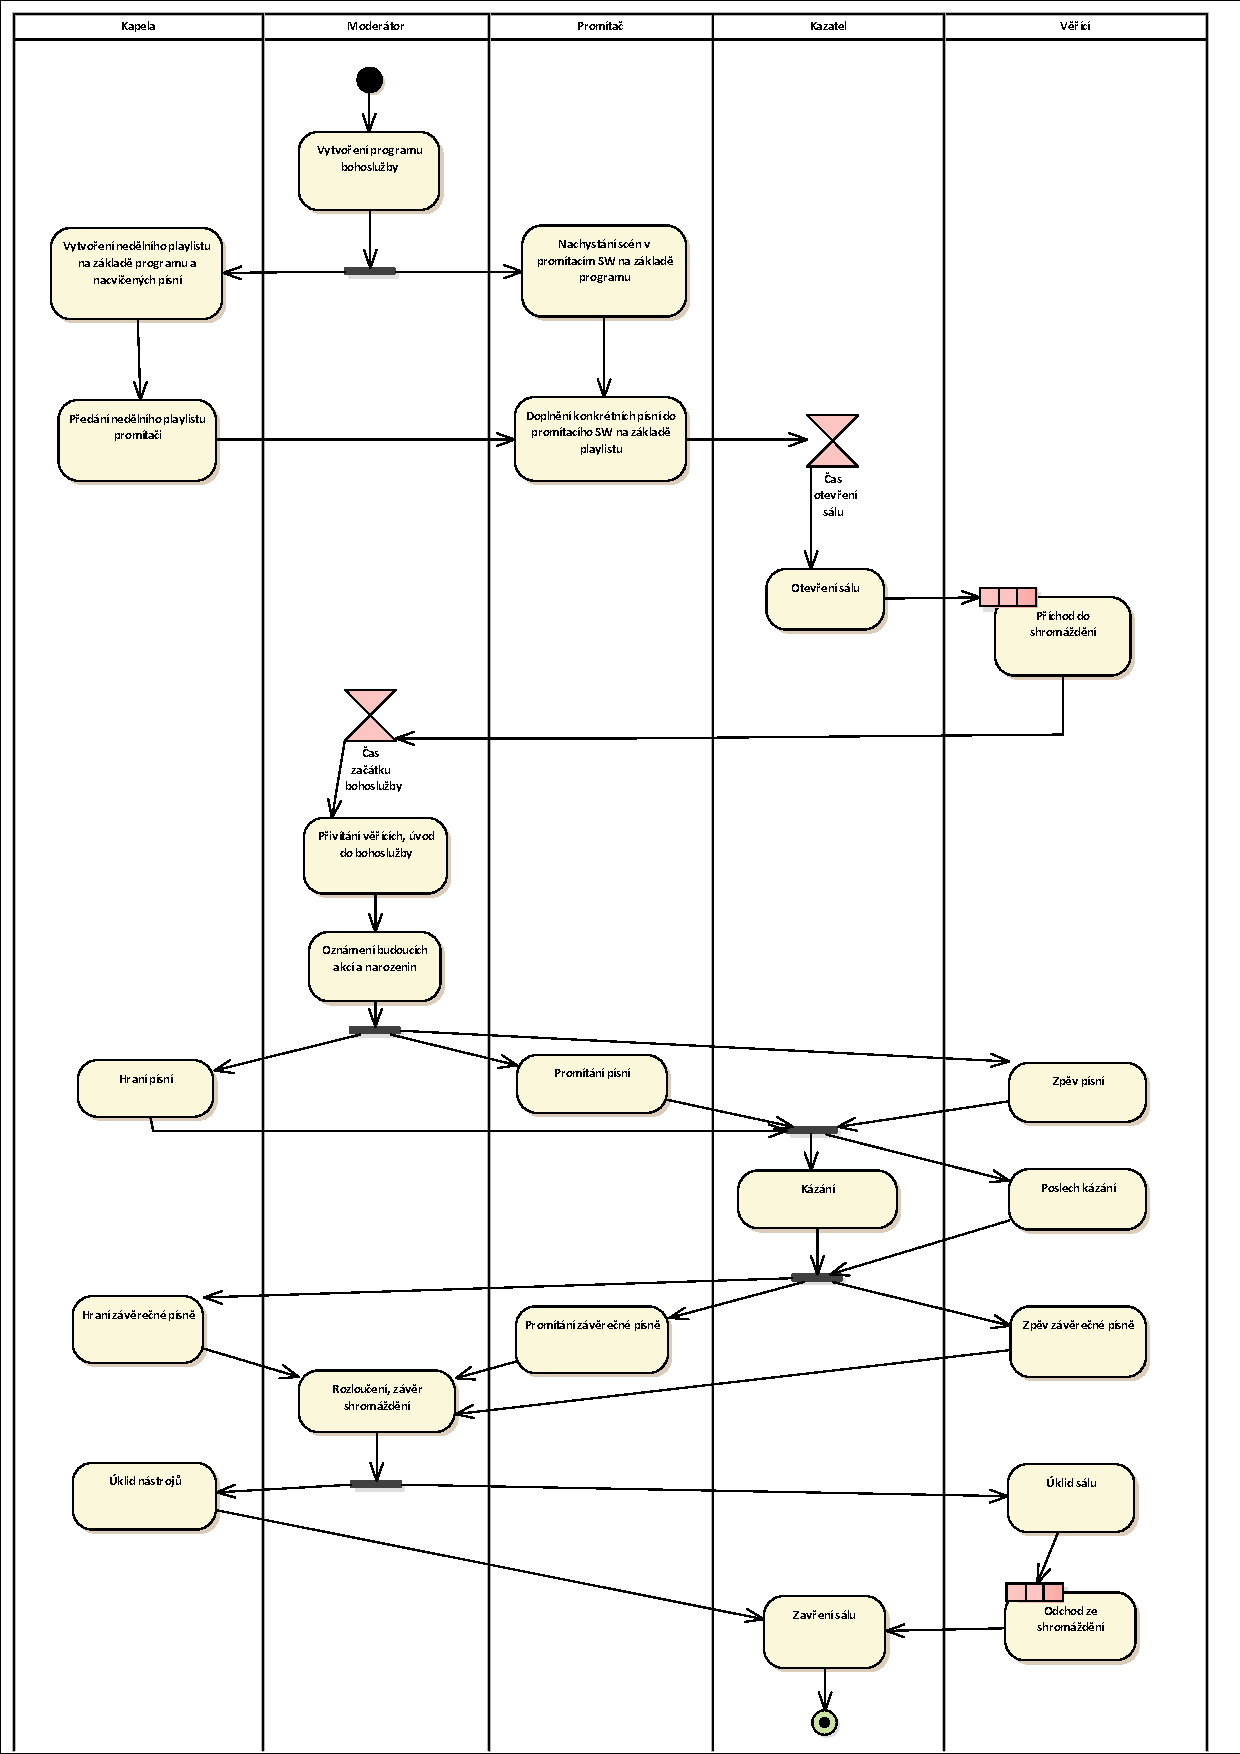
\includegraphics[width=\textwidth]{images/2-analyza/2-1-nedelni-shromazdeni.pdf}
    \caption{Diagram aktivit průběhu nedělního shromáždění}
\end{figure}

\begin{figure}
    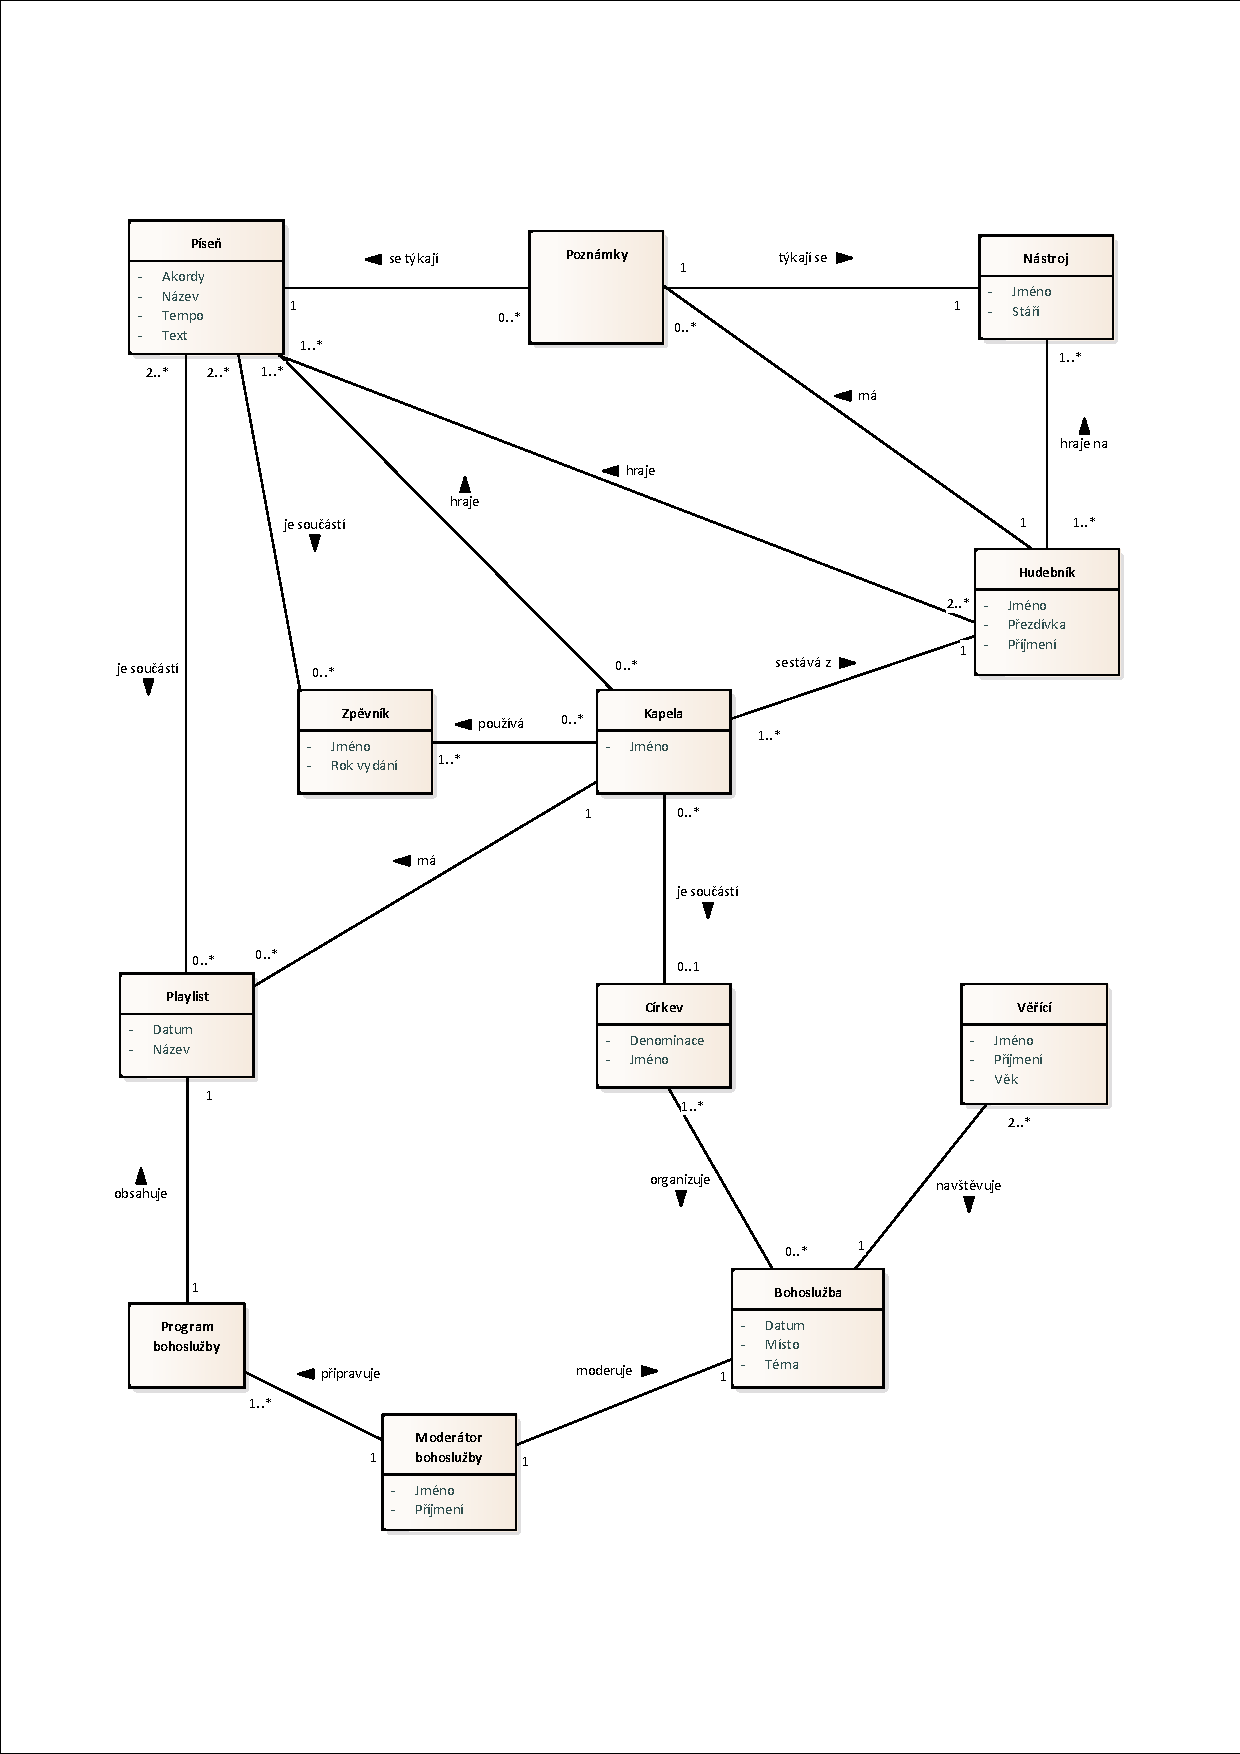
\includegraphics[width=\textwidth]{images/2-analyza/2-2-domenovy-model.pdf}
    \caption{Doménový model náboženských shromáždění}
\end{figure}

\subsection{Apoštolská církev Agapé Český Těšín}
\label{ac-agape}

Apoštolská církev Agapé Český Těšín (dále jen AC Agapé) \cite{ac-agape} se skládá z přibližně 70 členů, z~nichž třetinu tvoří Poláci. AC Agapé se schází ve staré židovské synagoze v Českém Těšíně. Synagoga je vybavena připojením k internetu, dataprojektorem a počítačem s operačním systémem Windows 10. Na bohoslužbě se běžně zpívá přibližně 10 až 15 písní. Střídají se zde dvě skupiny hudebníků -- Jóšafat a Agapebend, které čítají každá přibližně 5--10 členů. Každá skupina má svůj vlastní zpěvník o přibližně 100 písních s tím, že existují písně, které jsou v obou zpěvnících, každá skupina je ale hraje v jiném tempu, s jiným textem nebo v jiném jazyce. Zpěvníky jsem v~roce 2017 převedl do digitální podoby do formátu OpenSong \cite{open-song-format}.

Kromě nedělní bohoslužby se zde věřící scházejí také v neformálních domácích skupinách. Program domácích skupin není pevně dán, většinou je zde ale přítomen alespoň jeden hudebník, který zajistí blok 3--5 písní. Domácnosti jsou vybaveny připojením k internetu a televizí podporující technologie pro zrcadlení obrazovky. Písně jsou vybírány \uv{na přání} věřících ze zpěvníku skupiny, ze které je právě přítomný hudebník.

\subsection{Křesťanský sbor Český Těšín}
\label{krsb-tesin}

Křesťanský sbor Český Těšín (dále jen KřSb Český Těšín) \cite{krsb-tesin} se skládá z přibližně 70 členů. KřSb Český Těšín se schází ve vlastní budově zrekonstruovaného dětského centra v Českém Těšíně, která je vybavena připojením k internetu, dataprojektorem a počítačem s operačním systémem Windows 10. V průběhu bohoslužby se běžně zpívají 3 písně, kromě těchto písní se zde ale navíc vyskytuje systém \uv{podávání písní}. Každou neděli je tak kromě skupiny hudebníků určena navíc skupina klavíristů, kteří pokrývají dva zde používané zpěvníky - Písně nového života (dále jen PNŽ) a Gloria, každý čítající přibližně 500 písní. Věřící pak mají možnost z jednoho z těchto zpěvníků vybrat libovolné písně, které jsou hudebníkem zahrány, přičemž shromáždění zpívá sborově (bez sólisty u mikrofonu).

Kromě nedělní bohoslužby se v budově KřSb Český Těšín také v pátek večer setkává klub mládeže Přístav \cite{krsb-pristav}. Přístav je zaměřen na věkovou skupinu 13--19 let, od čehož se odvíjí i program setkání: začíná se hrou, následuje blok 3--4 písní, které připravuje skupina hudebníků Přístav Worship, 30 minutové zamyšlení na témata aktuální pro věkovou skupinu mladých a diskuze nad tématem spojené s konzumací jídla. Skupina Přístav Worship se skládá z 8 hudebníků a její zpěvník, čistě v digitální formě, obsahuje přibližně 30 písní.

\subsection{Křesťanský sbor Pyšely}
\label{krsb-pysely}

Křesťanský sbor Pyšely (dále jen KřSb Pyšely) \cite{krsb-pysely} se skládá z přibližně 30 členů. KřSb Pyšely se schází v budově Rodinného centra Zajíček o.s. v Zaječicích. Tato budova je vybavena připojením k internetu, není ale vybavena ani počítačem, ani dataprojektorem. Na bohoslužbě se běžně zpívá přibližně 5 písní, které má na starost jediné uskupení hudebníků, které zde působí. Zdejší hudební uskupení používá zpěvník v digitální a papírové podobě obsahující přibližně 30 písní.

\section{Funkční požadavky}

Jak jsem již nastínil v kapitole \nameref{uvod}, ve své práci se zabývám dvěma problémy, z čehož vyplývají dvě různé skupiny funkčních požadavků. Při porovnávání stávajících řešení budu tedy porovnávat zvlášť, zda systém splňuje požadavky týkající se koordinace zpěvu věřících a hudebního doprovodu (písmeno K) a požadavky týkající se přípravy písní (písmeno P).

\subsection{K1 Zobrazení textu aktuálně hrané písně}
\label{zobrazeni-textu-hrane-pisne}

Věřící v průběhu zpěvu písní potřebují vědět, kterou píseň hudební doprovod aktuálně hraje. Zkušení věřící, kteří jsou členy náboženského shromáždění dlouho, texty písní již znají, jsou tedy schopni aktuální hranou píseň rozpoznat samostatně. Nově příchozí věřící však texty písní neznají a potřebují tedy zjistit a vidět text aktuálně hrané písně.

\subsection{P1 Zobrazení seznamu písní a detailu písně}
\label{zobrazeni-seznamu-pisni-detailu}

Hudební doprovod potřebuje vidět seznam všech písní. U každé písně pak systém musí zobrazit její akordy a text včetně možnosti úpravy velikosti písma tak, aby byly text i akordy čitelné. Jelikož někteří členové hudebního doprovodu  pouze zpívají, systém by měl umožnit skrytí akordů. Pro členy hudebního doprovodu by pak měl systém poskytnout možnost nastavení transpozice akordů.

\subsection{P2 Organizace písní do zpěvníků}
\label{organizace-pisni-do-zpevniku}

Hudební doprovod potřebuje způsob, kterým zorganizuje jednotlivé písně do zpěvníků tak, aby byl schopen písně identifikovat jejich číslem ve zpěvníku a mohl ve zpěvníku efektivně vyhledávat podle tohoto čísla, případně názvu písně.

Název písně ale není spolehlivým identifikátorem. Často se stává, že různí členové hudebního doprovodu mají stejnou píseň zapamatovanou pod jiným názvem -- systém by měl tedy zvládnout také vyhledávání podle textu písně.

\subsection{P3 Správa písní a zpěvníků}
\label{sprava-pisni-zpevniku}

Hudební doprovod písně zpívané a hrané při náboženských shromážděních občas obměňuje. Přibližně jednou za 2 až 3 měsíce proběhne také přeuspořádání písní ze starých zpěvníků do~no\-vých. Systém proto musí umožnit hudebníkům úpravu, přidávání a odebírání písní a vedoucímu také vytváření, úpravu, odebírání zpěvníků a přesouvání písní mezi jednotlivými zpěvníky.

\subsection{P4 Správa playlistu}
\label{sprava-playlistu}

Z analýzy vyplynulo, že hudební doprovod pravidelně nejen na nedělní shromáždění připravuje seznam písní, které bude hrát -- playlist. Systém tak musí umožnit přidání písní do playlistu, jejich odebrání a změnu pořadí písně v rámci playlistu.

\subsection{P5 Správa členů kapely}
\label{sprava-clenu-kapely}

V systému bude působit více hudebních uskupení z různých náboženských shromáždění. Je proto nutné, aby systém umožnil každému uskupení mít oddělený zpěvník a oddělené písně, které budou přístupné pouze členům daného uskupení.

Z rozhovorů vyšel požadavek na rozdílná práva pro vedoucího, který může přidávat, upravovat a odebírat členy, zpěvníky a písně; hudebníka, který může upravovat pouze písně a zpěváka, který nemá právo upravovat.

\subsection{P6 Správa poznámek k písním}
\label{sprava-poznamek}

Členové hudebního doprovodu mají k jednotlivým písním různé poznámky. Zpěváci si k jednotlivým částem písně zaznamenávají, kde zpívají první a druhý hlas, hudebníci si naopak zaznamenávají kdy mají sólo nebo jaký použít rejstřík na svém hudebním nástroji. Tyto poznámky se vztahují pouze ke konkrétnímu členovi a ostatní členové ani vedoucí by je neměli vidět.

\subsection{P7 Synchronizace písní a zpěvníků}
\label{synchronizace-pisni-zpevniku}

Mezi členy hudebního doprovodu musí být synchronizovány jednotlivé písně a zpěvníky. Z rozhovorů s jednotlivými členy hudebních uskupení jsem zjistil, že jsou uskupení rozmanitou skupinou -- někteří členové mají zařízení s operačním systémem iOS, někteří macOS, Android a někteří mobilní zařízení ani nevlastní. Nezávisle na platformě, pro kterou bude systém vytvořen, musí systém umožnit synchronizaci písní a zpěvníků i na ostatní platformy, včetně možnosti tisku písní pro členy, kteří nevlastní žádné mobilní zařízení.

\subsection{P8 Synchronizace playlistu}
\label{synchronizace-playlistu}

Sestavený playlist musí vedoucí hudebního doprovodu před začátkem shromáždění předat jednotlivým hudebníkům. Systém musí tedy vedoucímu umožnit nahrání playlistu a jednotlivým členům hudebního doprovodu pak jeho stažení.

\section{Nefunkční požadavky}

V průběhu rozhovorů členové hudebního doprovodu vznesli také následující nefunkční požadavky na aplikaci:

\subsection{N1 Offline funkčnost (alespoň v režimu pro čtení)}
\label{offline-funkcnost}

V létě náboženská shromáždění pořádají letní tábory, které se často konají v přírodě, kde není dostupné připojení k internetu. Aplikace tak musí fungovat i bez přístupu k internetu, a to alespoň pro zobrazení playlistu, zpěvníků a písní. Úpravy bude provádět především vedoucí hudebního doprovodu, a to doma. Z průzkumu Českého statistického úřadu vyplývá, že je dnes více než 80 \% domácností připojeno k internetu. \cite{internet-usage-czechia} Podpora úprav bez připojení k internetu tak není nezbytně nutná a používání aplikace pouze zpříjemní.

\subsection{N2 Mobilní aplikace pro systémy iOS a macOS}

Vzhledem k tomu, že bude aplikace používána nejen v budovách náboženských shromáždění, ale také v domácnostech nebo v přírodě, musí se jednat o aplikaci pro mobilní telefon.

Z průzkumu mezi členy hudebního doprovodu vyplynulo, že bude nejvýhodnější aplikace pro systém iOS a macOS, jelikož právě tyto systémy používají vedoucí a více než polovina členů.

\subsection{N3 API rozhraní pro budoucí rozšířitelnost}

Z analýzy vyplývá, že v hudebních doprovodech existuje nezanedbatelné množství členů, kteří vlastní mobilní telefon s operačním systémem Android. Členové hudebních doprovodů se také zmínili o možnosti budoucího rozšíření zpěvníku do webové verze. Systém tak musí využívat API rozhraní, aby bylo toto případné budoucí rozšíření co nejjednodušší.

\subsection{N4 Přístupné a intuitivní rozhraní aplikace}

Většina členů hudebního doprovodu, tedy hlavní cílové skupiny uživatelů aplikace, je starší než 40 let. Aplikace tedy musí mít jednoduché a intuitivní rozhraní, aby se v ní vyznali i starší uživatelé, kteří nemají bohaté zkušenosti s používáním mobilních zařízení. Vzhledem k vyššímu věku některých členů hudebního doprovodu je také nutné, aby aplikace podporovala nastavení větší velikosti textu.

\subsection{N5 Podpora češtiny a polštiny}

Hudební uskupení z náboženských shromáždění, pro které je aplikace určena, jsou složena z~nezanedbatelné části také z polsky mluvících obyvatel. Aplikace tedy musí umožnit volbu jazyka a to minimálně mezi českým a polským jazykem.

\subsection{N6 Cena}

V náboženských shromážděních je obecně problém s finančním zajištěním čehokoliv. Většina služeb se tak opírá o dobrovolnost věřících. Jediný, kdo bývá placený, a to jen v některých shromážděních, je kazatel, který práci v shromáždění věnuje celý týden. Aplikace tedy musí být vytvořena zadarmo a měla by mít co nejnižší provozní náklady a náklady na údržbu.

\section{Stávající řešení koordinace zpěvu a doprovodu}

Problémy přípravy a koordinace zpěvu věřících a hudebního doprovodu náboženská shromáždění provází od jejich vzniku, z čehož vyplývá, že se o jejich řešení snaží věřící už dlouhá staletí.

Problém koordinace zpěvu věřících a hudebního doprovodu je v dnešní době řešen především třemi způsoby: Lidská paměť, Papírový zpěvník a Promítač. Tyto způsoby porovnám a zhodnotím, zda jsou pro náboženská shromáždění dostačující.

\subsection{Lidská paměť}

Velká část věřících a někteří hudebníci už znají texty a akordy jednotlivých písní nazpaměť -- při zpěvu písní tedy během prvních slov aktuálně hranou píseň poznají. Toto řešení je vhodné v~případě, kdy písní není mnoho, často se neobměňují a do náboženských shromáždění nepřichází mnoho nových věřících. Věřící také musí mít dobrou paměť, aby si texty písní pamatovali. Toto řešení z analyzovaných shromáždění používají jednotliví věřící, pro všechny ale není použitelné.

\subsection{Papírový zpěvník}

V historii nejčastěji používané řešení, od kterého se v posledních letech začíná ustupovat. Každé\-mu členu shromáždění je dán papírový zpěvník, ve kterém jsou všechny písně seřazeny podle jejich čísla ve zpěvníku. Hudební doprovod pak oznámí jméno písně, která je hrána a věřící si ji nalistují. Toto řešení je používáno ve shromáždění \nameref{krsb-pysely} a také při \uv{podávání písní} ve shromáždění \nameref{krsb-tesin}. Od řešení papírového zpěvníku se v poslední době ustupuje vzhledem k jeho vysoké ceně v případě velkého počtu věřících a také vzhledem k~obtížnosti úpravy jednou vytisknutého zpěvníku.

\subsection{Promítač}

Promítač je osoba, která promítá s pomocí dataprojektoru a promítacího programu text aktuálně hrané písně. Věřící při zpěvu písní sledují plátno, na kterém vidí text aktuálně hrané písně. V~dnešní době se jedná o nejčastěji používané řešení -- je vhodné pro libovolný počet věřících a písně v něm se dají libovolně upravovat. Jediným slabým článkem tohoto řešení je promítač samotný -- často tuto roli dostávají mladší věřící, kteří se v průběhu zpěvu písní zahledí do~mobilního telefonu a píseň zapomenou přepnout.

Na trhu jsou k dispozici různé promítací programy. Nejčastěji používaným je OpenSong. Ten umožňuje jednoduchou správu písní, organizaci do zpěvníků, správu playlistu a promítání aktuálně hrané písně. OpenSong využívá OpenSong formát \cite{open-song-format}, který je jednoduše čitelný jak lidským okem, tak strojově (jedná se o XML). OpenSong je používán ve shromáždění \nameref{ac-agape}.

Druhým nejčastěji používaným promítacím programem je OpenLP. Ten oproti OpenSongu umožňuje také promítání videí a prezentací včetně jejich zařazení do playlistu. OpenLP používá OpenLyrics formát \cite{open-lyrics-format}, který je lidsky obtížně čitelný, strojově se ale stále jedná o čitelné XML. OpenLP je používáno ve shromáždění \nameref{krsb-tesin}.

\subsection{Mobilní aplikace}

V rámci analýzy jsem také hledal mobilní aplikace, které by umožňovaly synchronizaci písní mezi hudebním doprovodem a věřícími, žádnou takovou aplikaci jsem ale nenašel. Z rozhovoru s~členy hudebního doprovodu jsem navíc zjistil, že by taková aplikace pro shromáždění ani neměla velký přínos -- někteří věřící nechtějí nebo nemůžou používat mobilní telefon a stávající řešení promítače věřícím plně vyhovuje.

\subsection{Shrnutí}

Z rozhovoru s členy hudebních uskupení v jednotlivých náboženských shromáždění vyplynulo, že jsou věřící v jednotlivých shromážděních se stávajícími řešeními koordinace zpěvu a hudebního doprovodu  spokojeni.

Při tvorbě mobilní aplikace zpěvníku pro náboženská shromáždění tedy nebudu vytvářet nová řešení problému koordinace zpěvu věřících a hudebního doprovodu, místo toho aplikaci napojím na stávající systémy, což bude řešeno ve funkčních požadavcích \nameref{sprava-playlistu} a \nameref{synchronizace-pisni-zpevniku}.

\section{Stávající řešení přípravy písní}

Problém přípravy písní je mnohem obecnější a řeší jej mnohé aplikace zpěvníku, které jsou dostupné na obchodech s aplikacemi pro operační systémy Android a iOS. Těchto řešení je velké množství, proto provedu analýzu pouze u těch, která náboženská shromáždění již používají nebo používaly a u těch řešení z obchodů s aplikacemi, které zhodnotím jako vhodné.

Pro tato řešení následně sestavím tabulku, ve které porovnám, v jaké míře splňují stanovené funkční a nefunkční požadavky.

\subsection{Papírový zpěvník}

Stejně jako u koordinace zpěvu věřících a hudebního doprovodu, i u přípravy písní je nejčastěji používaným řešením použití papírového zpěvníku. Jeho výhodou je neomezená funkčnost bez přístupu k internetu, jednoduchost a také možnost poznámek -- vytisknutý zpěvník si může hudebník bez problému popsat libovolnými poznámkami.

Papírový zpěvník ale přináší značné nevýhody -- není zde možnost úpravy textu písní nebo přidávání a odebírání písní ze zpěvníku. Příprava zpěvníku je náročná -- zpěvník musí být vytvořen, následně vytištěn a to v desítkách kusů. Pokud se hudebník rozhodne, že bude chtít hrát píseň z jiné tóniny, musí si k vytištěné písni poznamenat akordy v jiné tónině, což je v případě častých změn akordů značně nepřehledné. Náročné je také přidání nového člena -- musí se pro něj vytisknout nová kopie zpěvníku.

\subsection{Zpěvník v galerii telefonu}

Zejména mezi mladými hudebníky v náboženských shromážděních je velmi populární způsob zpěvníku ve formě sdílených fotografií na chatovací platformě. Každá konverzace odpovídá playlistu na jednu akci. Výhodou je velmi jednoduchý způsob přidání nového uživatele a správa oprávnění, nevýhodou je ale nemožnost použití takového řešení pro velký počet uživatelů a stejně jako v případě papírového zpěvníku zde chybí možnost úpravy stávajících písní nebo změny akordů v případě transpozice.

\subsection{OpenSongApp}

Aplikace OpenSongApp je dostupná na mobilní zařízení s operačním systémem Android. Umož\-ňuje jednoduchou správu písní, zpěvníků a playlistů v OpenSong formátu \cite{open-song-format}, je tedy plně kompatibilní s počítačovým promítacím programem OpenSong. Právě proto je aktivně používána v~shromáždění \nameref{ac-agape}.

Hlavní nevýhodou této aplikace je její omezení na operační systém Android. Druhou nevýho\-dou je synchronizace písní a playlistů mezi jednotlivými členy kapely a promítačem -- OpenSongApp samotná sice používá stejný formát jako OpenSong, neumožňuje ale synchronizaci samotnou. Písně je tedy třeba synchronizovat buď pomocí síťového úložiště nebo manuálně přes kabel, což je ale pro věkovou skupinu členů hudebního doprovodu často nesplnitelný úkol. OpenSongApp také neumožňuje správu uživatelů a kontrolu práv.

\subsection{Setlists}

Aplikace Setlists je dostupná pouze pro operační systém iOS. Setlists umožňuje správu playlistů a písní, její nevýhodou je vysoká cena (600 Kč na jedno zařízení), absence funkcionality zpěvníků, správy uživatelů. Rozhraní není příliš intuitivní a písně nelze jednoduše nahrát do aplikace. Toto řešení bylo jeden týden využíváno v \nameref{ac-agape}, ale příliš se neosvědčilo.

\subsection{Practice Books}

Aplikace Practice Books je dostupná pro operační systémy iOS a macOS. Umožňuje správu písní a zpěvníků a jejich synchronizaci mezi jednotlivými platformami. Její výhodou je jednoduché rozhraní a snadný způsob nahrání písní do aplikace.

Drobnou nevýhodou této aplikace je její cena, která ale není příliš vysoká -- 129 Kč na osobu. Mnohem zásadnějším problémem je ale absence playlistů, polštiny, chybějící správa členů kapely a oprávnění nebo možnost synchronizace mezi různými osobami. Aplikace také z nepochopitelných důvodů padá. Toto řešení bylo aktivně používáno v \nameref{ac-agape} během středečních domácích skupin, kdy vzhledem k tomu, že zde působil jeden hudebník nevadila absence playlistu, na nedělních shromážděních se ale příliš neosvědčila.

\subsection{Shrnutí}

Po provedení analýzy stávajících řešení jsem sepsal do tabulky, zda jednotlivá řešení splňují (A), částečně splňují (C), nesplňují (N) nebo nejsou relevantní (-) k stanoveným funkčním/nefunkčním požadavkům.

Z tabulky lze vidět, že neexistuje řešení, které by alespoň částečně splňovalo všechny funkční a nefunkční požadavky. Stávající řešení nesplňují funkční požadavek \nameref{sprava-clenu-kapely}, a velká část z nich má také problém s funkčním požadavkem \nameref{synchronizace-playlistu}.

\begin{table}[H]
\caption{Tabulka splnění funkčních požadavků stávajícími řešeními}
\begin{tabular}{|l||c|c|c|c|c|c|c|c|}
    \hline
    řešení & P1 & P2 & P3 & P4 & P5 & P6 & P7 & P8 \\
    \hline
    Papírový zpěvník           & A & A & C & C & N & A & N & N \\
    Zpěvník v galerii telefonu & N & N & N & A & A & N & C & A \\
    OpenSongApp                & A & A & A & A & N & A & C & C \\
    Setlists                   & A & N & C & A & N & N & C & C \\
    Practice Books             & A & A & A & N & N & N & C & N \\
    \hline
\end{tabular}
\end{table}

\begin{table}
\caption{Tabulka splnění nefunkčních požadavků stávajícími řešeními}
\begin{tabular}{|l||c|c|c|c|c|c|}
\hline
    řešení & N1 & N2 & N3 & N4 & N5 & N6 \\
    \hline
    Papírový zpěvník           & A & - & - & A & A & C \\
    Zpěvník v galerii telefonu & A & A & - & A & A & A \\
    OpenSongApp                & A & N & N & A & A & A \\
    Setlists                   & A & A & N & N & N & N \\
    Practice Books             & A & A & N & A & N & C \\
    \hline
\end{tabular}
\end{table}

Po domluvě s členy hudebního doprovodu v jednotlivých shromážděních jsem se tedy rozhodl implementovat mobilní aplikaci, která bude řešit problém přípravy zpěvu věřících a hudebního doprovodu. Problém koordinace zpěvu věřících a hudebního doprovodu bude nadále řešen promítačem a papírovým zpěvníkem, nově vzniklá aplikace ale s těmito řešeními bude kompatibilní.
